\documentclass[12pt, a4paper, oneside]{ctexart}
\usepackage{amsmath, amsthm, amssymb, bm, color, graphicx, geometry, mathrsfs,extarrows, braket, booktabs, array, xcolor, fontspec, appendix, float, subfigure, wrapfig, enumitem, titlesec}
\usepackage[colorlinks,linkcolor=red,anchorcolor=blue,citecolor=blue,urlcolor=blue,menucolor=black]{hyperref}

%%%% 设置中文字体 %%%%
% fc-list -f "%{family}\n" :lang=zh >d:zhfont.txt 命令查看已有字体
\setCJKmainfont[
    BoldFont=方正黑体_GBK,  % 黑体
    ItalicFont=方正楷体_GBK,  % 楷体
    BoldItalicFont=方正粗楷简体,  % 粗楷体
    Mapping = fullwidth-stop  % 将中文句号“.”全部转化为英文句号“.”,
]{方正书宋简体}  % !!! 注意在Windows中运行请改为“方正书宋简体.ttf” !!!
%%%% 设置英文字体 %%%%
\setmainfont{Minion Pro}
\setsansfont{Calibri}
\setmonofont{Consolas}

%%%% 设置代码块 %%%%
% 在vscode中使用minted需要先配置python解释器, Ctrl+Shift+P, 输入Python: Select Interpreter选择安装了Pygments的Python版本. 再在setting.json中xelatex和pdflatex的参数中加入 "--shell-escape", 即可
% TeXworks中配置方法参考: https://blog.csdn.net/RobertChenGuangzhi/article/details/108140093
\usepackage{minted}
\renewcommand{\theFancyVerbLine}{
    \sffamily\textcolor[rgb]{0.5,0.5,0.5}{\scriptsize\arabic{FancyVerbLine}}} % 修改代码前序号大小
% 加入不同语言的代码块
\newmintinline{cpp}{fontsize=\small, linenos, breaklines, frame=lines}
\newminted{cpp}{fontsize=\small, baselinestretch=1, linenos, breaklines, frame=lines}
\newmintedfile{cpp}{fontsize=\small, baselinestretch=1, linenos, breaklines, frame=lines}
\newmintinline{matlab}{fontsize=\small, linenos, breaklines, frame=lines}
\newminted{matlab}{fontsize=\small, baselinestretch=1, mathescape, linenos, breaklines, frame=lines}
\newmintedfile{matlab}{fontsize=\small, baselinestretch=1, linenos, breaklines, frame=lines}
\newmintinline{python}{fontsize=\small, linenos, breaklines, frame=lines, python3}  % 使用\pythoninline{代码}
\newminted{python}{fontsize=\small, baselinestretch=1, linenos, breaklines, frame=lines, python3}  % 使用\begin{pythoncode}代码\end{pythoncode}
\newmintedfile{python}{fontsize=\small, baselinestretch=1, linenos, breaklines, frame=lines, python3}  % 使用\pythonfile{代码地址}

%%%% 设置行间距与页边距 %%%%
\linespread{1.2}
\geometry{left=2.5cm, right=2.5cm, top=2.5cm, bottom=2.5cm}
% \geometry{left=1.84cm,right=1.84cm,top=2.18cm,bottom=2.18cm}  % 更小的页边距

%%%% 定理类环境的定义 %%%%
\newtheorem{example}{例}            % 整体编号
\newtheorem{theorem}{定理}[section] % 定理按section编号
\newtheorem{principle}{原理}[section] % 定理按section编号
\newtheorem{definition}{定义}[section]
\newtheorem{axiom}{公理}
\newtheorem{property}{性质}
\newtheorem{proposition}{命题}
\newtheorem{lemma}{引理}
\newtheorem{corollary}{推论}
\newtheorem{condition}{条件}
\newtheorem{conclusion}{结论}
\newtheorem{assumption}{假设}
\numberwithin{equation}{section}  % 公式按section编号 (公式右端的小括号)
\newtheorem{algorithm}{算法}

%%%% 自定义环境 %%%%
\newsavebox{\nameinfo}
\newenvironment{myTitle}[1]{
    \begin{center}
    {\makebox[0.8\linewidth][s]{\zihao{2}\bf #1}\\}
    \vspace{1ex}
    \zihao{4}\it
}{\end{center}}  % \begin{myTitle}{标题内容}作者信息\end{myTitle}
\newcounter{problem}  % 问题序号计数器
\newenvironment{problem}[1][]{\stepcounter{problem}\par\noindent\textbf{题目\arabic{problem}. #1}}{\smallskip\par}
\newenvironment{solution}[1][]{\par\noindent\textbf{#1解答. }}{\smallskip\par}  % 可带一个参数表示题号\begin{solution}{题号}
\newenvironment{note}{\par\noindent\textbf{注记. }}{\smallskip\par}
\newenvironment{remark}{\begin{enumerate}[label=\textbf{注\arabic*.}]}{\end{enumerate}}
\BeforeBeginEnvironment{minted}{\vspace{-0.5cm}}  % 缩小minted环境距上文间距
\AfterEndEnvironment{minted}{\vspace{-0.2cm}}  % 缩小minted环境距下文间距

%%%% 自定义段落开头序号,间距 (titlesec) %%%%
% 中文序号:\zhnum{section}, 阿拉伯序号:\arabic
\titleformat{\section}{\Large\bfseries}{\arabic{section}}{1em}{}[]
\titlespacing{\section}{0pt}{1.2ex plus .0ex minus .0ex}{.6ex plus .0ex}
\titlespacing{\subsection}{0pt}{1.2ex plus .0ex minus .0ex}{.6ex plus .0ex}
\titlespacing{\subsubsection}{0pt}{1.2ex plus .0ex minus .0ex}{.6ex plus .0ex}

%%%% 图片相对路径 %%%%
\graphicspath{{figures/}} % 当前目录下的figures文件夹, {../figures/}则是父目录的figures文件夹
\setlength{\abovecaptionskip}{-0.2cm}  % 缩紧图片标题与图片之间的距离
\setlength{\belowcaptionskip}{0pt} 

%%%% 缩小item,enumerate,description两行间间距 %%%%
\setenumerate[1]{itemsep=0pt,partopsep=0pt,parsep=\parskip,topsep=5pt}
\setitemize[1]{itemsep=0pt,partopsep=0pt,parsep=\parskip,topsep=5pt}
\setdescription{itemsep=0pt,partopsep=0pt,parsep=\parskip,topsep=5pt}

%%%% 自定义公式 %%%%
\everymath{\displaystyle} % 默认全部行间公式, 想要变回行内公式使用\textstyle
\DeclareMathOperator*\uplim{\overline{lim}}     % 定义上极限 \uplim_{}
\DeclareMathOperator*\lowlim{\underline{lim}}   % 定义下极限 \lowlim_{}
\DeclareMathOperator*{\argmax}{arg\,max}  % 定义取最大值的参数 \argmax_{}
\DeclareMathOperator*{\argmin}{arg\,min}  % 定义取最小值的参数 \argmin_{}
\let\leq=\leqslant % 简写小于等于\leq (将全部leq变为leqslant)
\let\geq=\geqslant % 简写大于等于\geq (将全部geq变为geqslant)
\DeclareRobustCommand{\rchi}{{\mathpalette\irchi\relax}}
\newcommand{\irchi}[2]{\raisebox{\depth}{$#1\chi$}} % 使用\rchi将\chi居中

%%%% 一些宏定义 %%%%
\def\bd{\boldsymbol}        % 加粗(向量) boldsymbol
\def\disp{\displaystyle}    % 使用行间公式 displaystyle(默认)
\def\tsty{\textstyle}       % 使用行内公式 textstyle
\def\sign{\text{sign}}      % sign function
\def\wtd{\widetilde}        % 宽波浪线 widetilde
\def\R{\mathbb{R}}          % Real number
\def\N{\mathbb{N}}          % Natural number
\def\Z{\mathbb{Z}}          % Integer number
\def\Q{\mathbb{Q}}          % Rational number
\def\C{\mathbb{C}}          % Complex number
\def\K{\mathbb{K}}          % Number Field
\def\P{\mathbb{P}}          % Polynomial
\def\E{\mathbb{E}}          % Exception
\def\d{\mathrm{d}}          % differential operator
\def\e{\mathrm{e}}          % Euler's number
\def\i{\mathrm{i}}          % imaginary number
\def\re{\mathrm{Re}}        % Real part
\def\im{\mathrm{Im}}        % Imaginary part
\def\res{\mathrm{Res}}      % Residue
\def\ker{\mathrm{Ker}}      % Kernel
\def\vspan{\mathrm{vspan}}  % Span  \span与latex内核代码冲突改为\vspan
\def\L{\mathcal{L}}         % Loss function
\def\O{\mathcal{O}}         % big O notation
\def\wdh{\widehat}          % 宽帽子 widehat
\def\ol{\overline}          % 上横线 overline
\def\ul{\underline}         % 下横线 underline
\def\add{\vspace{1ex}}      % 增加行间距
\def\del{\vspace{-1.5ex}}   % 减少行间距

%%%% 正文开始 %%%%
\begin{document}

%%%% 以下部分是正文 %%%%  
\clearpage
\begin{myTitle}{西安交通大学学生答题纸}
\makebox[\linewidth][s]{学生姓名:\underline{\ 吴天阳\ }学号:\underline{\ 2204210460\ }所在班级:\underline{\ 强基数学002\ }}\\[1ex]
\makebox[\linewidth][s]{所属学院:\underline{\ 数学与统计\ }考试课程:\underline{《历史上最伟大的10个方程》导读}}\\[1ex]
\makebox[\linewidth][s]{考试时间:\underline{\today}考试成绩:\underline{\hspace{10em}}}
\end{myTitle}

这篇课程报告是对\textbf{爱因斯坦质能方程}的理解,
本文将尽力详细介绍每个公式的推导过程,
并给出每个公式具体物理意义的理解。由于我并不是物理专业学生,缺少对完整理论的学习,
所以对公式含义的理解可能有所偏差,请老师纠正。

由于质能方程是狭义相对论的结论,所以我先介绍基于狭义相对论推导出的和时空相关结论,分别包含:
时间膨胀、长度收缩、Lorentz变换、时空图及光锥,再介绍质能方程和能量动量关系,其实本文主要部分集中在如何理解狭义相对论中的时空观。
\section{狭义相对论——时空观}
首先,需要引入一些经典力学下的定义,基于这些定义我们才能引出爱因斯坦的狭义相对论。
\begin{definition}
没有任何加速度的参考系称为\textbf{惯性参考系(Inertia frame of reference)}。
\end{definition}
\begin{theorem}[惯性原理,牛顿第一定理]
    当物体不受外力作用时,在惯性参考系下,该物体一定\textbf{保持静止或者匀速运动状态}。
\end{theorem}
不难发现,对于两个惯性参考系,它们相互之间只有静止和匀速运动两个状态。
\begin{theorem}[相对性原理, principle of relativity]
    所有的物理定律在任何一个惯性参考系中都保持一致。
\end{theorem}
相对性原理最初由Galileo于1632年在其著作《关于托勒密和哥白尼两大世界体系的对话》提出,该书为避免宗教问题,没有直接地以定义形式阐述观点,
而是通过Salviati、Sagredo和Simplicio三人对话的方式展开,故事中Salviati提出一个实验,在一个匀速直线运动的密封船舱内,
无论你做什么实验,都无法判断出船当前的状态是运动还是静止的。这间接的说明了,无法通过任何物理实验区分两个惯性参考系,
即\textbf{惯性参考系中物理定律的一致性}。

\textbf{狭义相对论(Special Relativity)}之所以称为“狭义”(或者称之为“特殊”),原因就是在于其所有假设都建立在相对性原理之上,
所有的运动都相对于惯性参考系。

\subsection{光速一致性}
当时那个时代,通过Maxwell方程计算可以得到电磁波的传播速度和光速正好相等,
所以人们猜测光也是一种电磁波,并认为一定存在一种用于承载电磁波的介质,
人们将其称为\textbf{以太(aether)}。

我们可以通过一个假象实验来类比以太和光,假设存在一个以速度$v$进行匀速直线运动的敞篷车,静止的状态下空气中的声速为$v'$,
如果车上的人沿着$v$的方向发出声波,那么车上的人测量得到的声速为$v'-v$,但是他们还是不能判断自己是否是运动的,
因为他们可以说空气沿着速度$-v$的方向匀速直线运动,相对性理论仍然成立。

我们将这个实验中的空气换成以太,声波换成光波,而汽车则换成地球,这个实验就是著名的\textbf{迈克耳孙-莫雷实验}。
假设以太存在,那么地球和以太之间一定存在相对速度,则光在某个方向上一定存在速度差异,
但是该实验结果表明,在各个方向上测得的光速不变,从而相对性原理仍然成立。

换句话说,如果狭义相对论的相对性理论基础成立,在任意惯性参考系下光速都为常量,我们将其记为$c$。
通过光速一致性这个条件,我们可以推导出更多推论。

\subsection{时间膨胀}
\begin{definition}
    \textbf{时间膨胀(Time Dilation)}是指在相对运动的参考系中的观察者,观察静止参考系中发生的相同事件,其所用的时间间隔会延长
    (事件必须在当前参考系中的相同位置处发生)。反之亦然,处于静止参考系中的观察者,观察运动参考系中发生的相同事件,其所用的时间间隔也会延长。
\end{definition}
这里从一个实验简单的对时间膨胀进行理解:设存在两个惯性参考系$\Sigma_1,\Sigma_2$,
从$\Sigma_1$观察$\Sigma_2$二者相对速度为水平方向$v$米每秒。
两个参考系中分别存在一个完全相同的水平平行反光镜,反光镜之间间距$L$米,有一束光在镜子中往返运动,每次抵达下底面时,时钟向前走一步“嘀嗒”。
下面我们计算在$\Sigma_1$中观察$\Sigma_2$的时钟,他的时钟会有什么变化。(这里必须要求光子回到出发点,就是为了满足\textbf{事件必须在相同位置处发生}的条件)

首先,在$\Sigma_1$下,“嘀嗒”一次所需的时间为$2L/c$秒,记为$\Delta t$;
由于$\Sigma_2$水平方向具有速度$v$,所以从$\Sigma_1$中经过$\Delta t'$时间,观察$\Sigma_2$中的光束运动路径如下:
\begin{figure}[htbp]
    \centering
    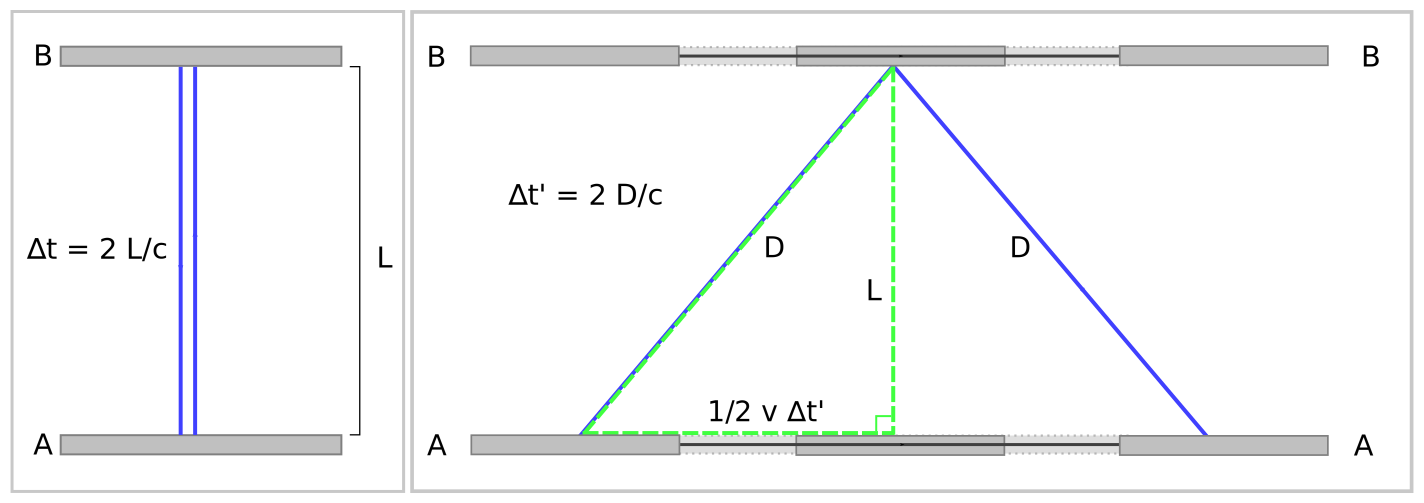
\includegraphics[width=1.0\linewidth]{Time-dilation-002-mod.png}
    \caption{在惯性参考系$\Sigma_1$下,左图为$\Sigma_1$中光子运动路径,右图为$\Sigma_2$中光子的运动路径}
    \label{figure-time-dilation}
\end{figure}

我们可以看到图\ref{figure-time-dilation}右图中绿色部分为直角三角形,利用勾股定理可得
\begin{equation}\label{eq-time-dilation}
    (c\Delta t'/2)^2 = L^2 + (v\Delta t'/2)^2\Rightarrow \Delta t' = \frac{2L/c}{\sqrt{1-\frac{v^2}{c^2}}} = \frac{\Delta t}{\sqrt{1-\frac{v^2}{c^2}}} = \gamma \Delta t
\end{equation}
其中$\gamma = \frac{1}{\sqrt{1-\frac{v^2}{c^2}}}$为Lorentz系数。从式\ref{eq-time-dilation}可以看出,$\Sigma_2$中的时间相对于$\Sigma_1$变长了$\gamma$倍;
注意这里的时间变化是相对的,也就是从$\Sigma_2$的角度看$\Sigma_1$中的时间也变长了$\gamma$倍。

有大量实验可以证明时间膨胀的存在,在太空中存在大量被地球吸附的粒子,这些粒子与大气中的某些原子核发生碰撞后会产生一种寿命极短的粒子,它被称为$\mu$粒子,
在静止状态下$\mu$粒子的半衰期时间为$2.20\mu s$,如果没有时间膨胀,那么所有的$\mu$粒子基本无法在地球表面被检测到。
但是有些$\mu$粒子的速度可以接近光速,通过研究发现$\mu$粒子的半衰期时间和速度成正相关关系,和时间膨胀所预测的一致。

\subsection{长度收缩}
我们可以进一步讨论由时间膨胀所导致的\textbf{长度收缩},也就是高速运动会导致不同惯性参考系中时空的形变,物体速度越快,两点的空间距离越短。

还是用上述例子进行解释,从$\mu$粒子自身看自己的静止衰变时间只有$2.20\mu s$,因此$\mu$粒子角度看地球的移动距离为
\begin{equation}
    L = v\Delta t = 0.95\times 3\times 10^8\times 2.20\times 10^{-8} = 0.627\ km
\end{equation}
但从地球上观察者角度看速度为$0.95c$运动的$\mu$粒子的衰变时间为$7.05\mu s$(由时间膨胀计算可得),因此从地球上观察者角度看$\mu$粒子的运动距离为
\begin{equation}
    L_0 = v\Delta t' = 0.95\times 3\times 10^8\times 7.05\times 10^{-8} = 2.01\ km
\end{equation}

首先我们给出静止长度的定义:
\begin{definition}
    静止长度(Proper Length)$L_0$是在\textbf{静止参考系}下观察两点之间的距离。(静止和运动是相对的,所以不妨令其中一个参考系是静止的即可)
\end{definition}
基于静止长度我们可以给出长度收缩的定义
\begin{definition}
    \textbf{长度收缩(Length Contraction)}是指在\textbf{相对运动参考系}下测量物体\textbf{沿着运动方向的长度}相对于其静止时长度的减少量:
    \begin{equation}
        L = L_0\sqrt{1-\frac{v^2}{c^2}} = L_0/\gamma
    \end{equation}
    其中$L_0$为物体的静止长度,$L$为物体在以速度$v$运动的参考系下观测到的长度。
\end{definition}
\begin{proof}
    利用物体在不同参考系下具有相同速度和时间膨胀可得
    \begin{equation}
        v = \frac{L_0}{\Delta t'} = \frac{L}{\Delta t}\Rightarrow L = \frac{\Delta t}{\Delta t'}L_0 = L_0/\gamma
    \end{equation}
\end{proof}

\textbf{注意}:在定义中我们强调只有沿着运动方向的长度会发生收缩,但是在垂直于运动方向的长度会发生变化么?

结论是不会,这里可以通过一个思维实验用反证法对其进行简单理解,假如存在两个人A,B,A向着B以近光速运动,
两人手上着均平行着拿着一把垂直的长度为1m尺子,当A到达B所在的位置时,他们相互地会用自己画笔基于自己尺子的1m距离在对方的尺子上进行标记,如图\ref{fig-length-contraction}所示。
假设存在垂直方向上的长度收缩,那么A在B上标记的位置一定低于1m,那么因此B无法在A上进行标记,因为A的尺子长度小于1m无法标记;
但是由于运动是相对的,B理论上也可以在A上标记位置,同样也会低于1m,这与B无法在A上进行标记的结论矛盾。

综上,假设不成立,所以不能存在垂直方向上的长度收缩。

\begin{figure}[htbp]
    \centering
    \includegraphics[scale=1]{length_contraction.jpg}
    \caption{在垂直方向上不会发生长度收缩}
    \label{fig-length-contraction}
\end{figure}

\subsection{Lorentz变换}
通过上述结论,我们可以得到更一般的结论,\textbf{Lorentz变换(Lorentz Transformations)}给出了运动所导致时间和空间上的变换关系:
\begin{theorem}[Lorentz变换]
    \textbf{惯性时空参考系}是由时间$t$和空间$(x,y,z)$四个维度唯一表示的坐标系,记为$S=\{(t,x,y,z)\}$。

    设$S_1 = \{(t,x,y,z)\},S_2 = \{(t',x',y',z')\}$分别为两个惯性时空参考系,
    假设$S_2$相对$S_1$在$x$轴方向上以速度$v$匀速直线运动,
    由于运动是相对的,所以通常将$S_1$视为\textbf{静止参考系(Rest Frame)},$S_2$视为\textbf{运动惯性参考系(Moving Inertial Frame)}
    则从$S_1$到$S_2$的Lorentz变换为
\begin{equation}\label{eq-Lorentz}
    \begin{cases}
        t' = \gamma\left(t - \frac{vx}{c^2}\right),\\
        x' = \gamma(x-vt),\\
        y' = y,\\
        z' = z.
    \end{cases}\iff
    \begin{bmatrix}
        t'\\x'\\y'\\z'
    \end{bmatrix} = \begin{bmatrix}
        \gamma&v/c^2\gamma&0&0\\
        v\gamma&\gamma&0&0\\
        0&0&1&0\\
        0&0&0&1
    \end{bmatrix}
    \begin{bmatrix}
        t\\x\\y\\z
    \end{bmatrix}
\end{equation}
其逆变换为
\begin{equation}\label{eq-Lorentz-inv}
    \begin{cases}
        t = \gamma\left(t' + \frac{vx'}{c^2}\right),\\
        x = \gamma(x'+vt),\\
        y = y',\\
        z = z'.
    \end{cases}\iff
    \begin{bmatrix}
        t\\x\\y\\z
    \end{bmatrix} = \begin{bmatrix}
        \gamma&-v/c^2\gamma&0&0\\
        -v\gamma&\gamma&0&0\\
        0&0&1&0\\
        0&0&0&1
    \end{bmatrix}
    \begin{bmatrix}
        t'\\x'\\y'\\z'
    \end{bmatrix}
\end{equation}
\end{theorem}
\begin{proof}
    \textbf{观察}:
    \begin{enumerate}
        \item Lorentz变换本质上给出了某个的事件,在不同参考系下的时空位置变换关系。
        \item Lorentz逆变换就正好是将Lorentz变换中的速度反向$v\gets-v$,这正好和狭义相对论结论一致,值得注意的是,
        Lorentz推导该公式是基于以太存在假设下得到的结果,但却正好印证了狭义相对论从数学坐标变换上的正确性。
    \end{enumerate}

    \textbf{分析}:利用狭义相对论中不同参考系中\textbf{光速不变}和沿运动方向上的\textbf{长度收缩}出发进行推导;利用下文中介绍的时空图,
    将$ct$变量视为一个整体,就可以得到更简单的变换关系式,从而易于求出逆变换。

    由于在不同参考系中光速不变,我们假设存在一个光子在$0$时刻时从原点出发,在$S_1$中的$t$时刻下运动到$(x,y,z)$,
    对应地在$S_2$中观察到该光子也从原点出发,在$t'$时刻运动到$(x',y',z')$,在欧式空间下,二者应满足
    \begin{equation}\label{eq-light-moving}
        x^2+y^2+z^2 - c^2t^2 = 0,\quad x'^2+y'^2+z'^2 - c^2t'^2 = 0
    \end{equation}
    由存在沿运动方向距离膨胀的关系,可得($x'$量纲为静止距离$L_0$,$x$为在运动参考系下观察到的距离膨胀,和$L$保持相同量纲)
    \begin{equation}\label{eq-length-contraction}
        x = vt + x'\sqrt{1-v^2/c^2}\Rightarrow x' = \frac{x-vt}{\sqrt{1-\frac{v^2}{c^2}}} = \gamma(x-vt)
    \end{equation}
    又由于沿着垂直于运动方向的长度不发生变换,则$y'=y, z'=z$,将其带入\ref{eq-light-moving}式中可得
    \begin{equation}
        x^2-c^2t^2 = x'^2-c^2t'^2 \Rightarrow t' = \sqrt{\frac{x'^2-x^2}{c^2}+t^2} = \sqrt{\frac{\gamma^2(x-vt)^2-x^2+c^2t^2}{c^2}}
    \end{equation}
    化简可得$t' = \frac{t-vx/c^2}{\sqrt{1-\frac{v^2}{c^2}}} = \gamma(t-vx/c^2)$。综上可得Lorentz变换\ref{eq-Lorentz}式。
    
    逆变换只需求解\ref{eq-Lorentz}右侧变换矩阵的左上方的子矩阵求逆即可,记$\beta = v/c$,则不难发现
    \begin{equation}
        \begin{bmatrix}
            ct'\\x'
        \end{bmatrix} = \gamma\begin{bmatrix}
            1&-\beta\\-\beta&1
        \end{bmatrix}\begin{bmatrix}
            ct\\x
        \end{bmatrix}
    \end{equation}
    更巧妙的是
    \begin{equation}
        \gamma^2\begin{bmatrix}
            1&-\beta\\-\beta&1
        \end{bmatrix}\begin{bmatrix}
            1&\beta\\\beta&1
        \end{bmatrix} = \gamma^2\begin{bmatrix}
            1-\beta^2&0\\0&1-\beta^2
        \end{bmatrix} = \begin{bmatrix}
            1&0\\0&1
        \end{bmatrix} = I_2
    \end{equation}
    于是我们得到逆变换:
    \begin{equation}
        \begin{bmatrix}
            ct\\x
        \end{bmatrix}=\gamma\begin{bmatrix}
            1&\beta\\\beta&1
        \end{bmatrix}\begin{bmatrix}
            ct'\\x'
        \end{bmatrix}
    \end{equation}
    将右下角$y=y',z=z'$补全就可得到Lorentz逆变换\ref{eq-Lorentz-inv}式。
\end{proof}
\textbf{注意}:对Lorentz变换证明中距离膨胀\ref{eq-length-contraction}的$x,x'$必须理解清晰,静止距离$L_0$为什么是在运动参考系$S_2=\{(t',x',y',z')\}$下得到的?
主要需要弄清楚$L_0$是在哪个参考系下得到的,我们又究竟想在哪个参考系下对该长度进行计算。

还是以$\mu$粒子的移动距离相对地球上测量得到的距离缩短为例,在地球为参考系测量得到的距离为$L_0$,
如果我们想从$\mu$粒子视角下测量距离,则需要将$\mu$粒子的参考系视为静止的$S_1$,所以地球参考系是$S_2$以速度$v$相对其运动,
所以我们得到在另一个运动参考系中的固定长度$L_0$,在静止参考系下观察得到其距离膨胀为$L_0\sqrt{1-v^2/c^2}$。

\subsection{时空图及光锥}
在三维欧式空间中,设两个点$A(x_1,y_1,z_1),B(x_2,y_2,z_2)$,则两点的$\L_2$范数距离为
\begin{equation}
    (\Delta r)^2 = (\Delta x)^2 + (\Delta y)^2 + (\Delta z)^2 = (x_1-x_2)^2 + (y_1-y_2)^2 + (z_1-z_2)^2
\end{equation}
我们知道在欧氏变换(平移、旋转)下$AB$两点之间距离仍然相同,即欧氏变换是该度量下的保距变换。

同理,我们是否也能找到在Lorentz变换下定义的距离,使得Lorentz变换相对其也是保距变换?事实上可以,我们如下定义\textbf{时空间隔(Spacetime interval)}
\begin{equation}
    (\Delta s)^2 = (\Delta x)^2 + (\Delta y)^2 + (\Delta z)^2 - (c\Delta t)^2
\end{equation}
将Lorentz逆变换\ref{eq-Lorentz-inv}式带入,可得
\begin{equation}
\begin{aligned}
    (\Delta s)^2 =&\ \gamma^2(\Delta x'+c\beta\Delta t')^2 - \gamma^2(c\Delta t' + \beta\Delta x')^2\\
    =&\ \gamma^2\left((\Delta x')^2 + 2c\beta\Delta x'\Delta t' + \beta^2(c\Delta t')^2 - (c\Delta t')^2 - 2c\beta \Delta x'\Delta t' - \beta^2(\Delta x')^2\right)\\
    =&\ \gamma^2 \left((1-\beta^2)(\Delta x')^2 - (1-\beta^2)(c\Delta t')^2\right)\\
    =&\ (\Delta x')^2 - (c\Delta t')^2 = (\Delta s')^2
\end{aligned}
\end{equation}
所以时空间隔$(\Delta s)^2$就是$AB$两点间在Lorentz变换下的不变量,也是\textbf{在任意惯性参考系下的不变量}。
但是我们容易发现,时空间隔可以是是正数也可以是负数,那么为什么还能记为平方呢?物理学家通常将$(\Delta s)^2$视为一个整体处理,
而不会单独考虑$s$,而且在\textbf{Minkowski空间}中距离可以是负数(引入虚数单位$i$),这样表示应该只是为了和勾股定理进行类比。

那么$(\Delta s)^2$的正负性所具有的物理含义是什么呢?下面先引入时空图,从而才能对其有更好的理解。

我们将三维空间绘制在水平轴上,时间维度绘制在纵轴上,就可以得到时空图,如图\ref{fig-spacetime}所示,具体含义请见注释部分。
\begin{figure}[htbp]
    \centering
    \includegraphics[scale=0.38]{spacetime.png}
    \caption{\textbf{时空图(Space-time Graph)},其中\textbf{世界布(Worldsheet)}是空间中以速度$v$相对当前参考系进行运动的物体轨迹集合;
    \textbf{单事件(Single Event)}是相对当前参考系在时空中发生的事件;
    \textbf{世界线(Worldline)}是指在时空中的物体相对与当前参考系的运动轨迹。}
    \label{fig-spacetime}
\end{figure}

观察时空参考系我们可以发现这些性质:
\begin{enumerate}
    \item 由于每个参考系中位置是相对的,对于时空中\textbf{任意的一个向量都可以被平移到原点处}。
    \item 由于时空的相对性,\textbf{单独对一个单事件进行讨论是没有意义的}。
    \item 在世界线上的任何一点的\textbf{切线就是该物体的速度倒数}。
\end{enumerate}

有了时间图就能讨论不同位置处的$(\Delta s)^2$正负性,我们称时间图中$(\Delta s)^2=0$的曲面为\textbf{光锥(Light Cone)}
(如果纵坐标的单位为$ct$,则光锥的倾斜角为$45^\circ$),如下图所示
\begin{figure}[htbp]
    \centering
    \includegraphics[scale=1.0]{light_cone.jpg}
    \caption{蓝色的曲面为光锥,点A为当前参考系的原点,点B是在光锥上半区内的点,满足$(\Delta s)^2 < 0$,意味着事件B一定会在事件A的未来发生(在任何参考系下观察都是如此);
    点C是光锥之外的点,满足$(\Delta s)^2 > 0$,意味着事件C既可能在事件A前发生也可能在后发生,取决于参考系的选取。}
\end{figure}

\begin{itemize}
    \item $(\Delta s)^2 < 0$:图\ref{fig-spacetime}中处于光锥的内部,由$\Delta t$主导,我们称两个事件$AB$可以\textbf{类时分离(Timelike Separation)},
    假设$AB$的斜率为速度$v$,则作用速度$v$的Lorentz变换,即可得到$x_A=x_B,y_A=y_B,z_A=z_B$,所以这两个事件只保持时间发生顺序。
    \item $(\Delta s)^2 > 0$:图\ref{fig-spacetime}中处于光锥的外部,由$\Delta x,\Delta y,\Delta z$主导,我们称两个事件$AC$可以\textbf{类空分离(Spacelike Separation)},
    我们发现这里$AC$的速度$v$已经超过光速$c$,因此我们可以在速度为$1/v$的参考系下观察使得事件$AC$同时发生,甚至如果我们选择速度在$(1/v,c)$中的参考系,甚至可以颠倒事件的发生顺序,
    这也说明这两个事件只保持空间发生顺序。
    \item $(\Delta s)^2 = 0$:图\ref{fig-spacetime}中所有处于光锥上的事件$D$,我们称两个事件$AD$是\textbf{类光(lightlike)}的或\textbf{不可分离(Null Separation)}的,
    这表明事件$AD$的速度$v$正好就是光速,在任何参考系下进行观察,$AD$发生的时空顺序一定不变。
\end{itemize}

最后我们再讨论\textbf{时空图上的Lorentz变换},设$O'$相对于$O$沿$v\bd{e}_x$方向运动,由Lorentz变换可知
\begin{equation}
    \begin{cases}
        ct' = \gamma(ct) - \beta\gamma x,\\
        x' = -\beta\gamma(ct) + \gamma x.
    \end{cases}
\end{equation}
当$x' = 0$时,得到变换后$ct'$轴方向:
\begin{equation*}
0 = -\beta\gamma(ct) + \gamma x \Rightarrow ct = \frac{c}{v}x,
\end{equation*}
当$t' = 0$时,得到变换后$x'$轴方向:
\begin{equation*}
0 = \gamma(ct)-\beta \gamma x \Rightarrow ct = \frac{v}{c}x.
\end{equation*}
在图像中绘制结果如下:
\begin{figure}[htbp]
    \centering
    \includegraphics[scale=0.5]{spacetime_Lorentz_transform.png}
    \caption{时空图下的Lorentz变换,橙色坐标系为静止坐标系$O=\{ct,x\}$,蓝色坐标系为速度$v\bd{e}_x$的惯性运动坐标系$O'=\{ct',x'\}$,
    点$A$为一个事件,$\Delta t,\Delta x$分别为坐标系$O$下的时空位置,相对的$\Delta t',\Delta x'$为坐标系$O'$下的时空位置。
    红色直线为光锥。}
\end{figure}

通过时空图下的Lorentz变换图,我们可以非常直观地看出时间膨胀和长度收缩,不难验证$\Delta t / \Delta t' =\Delta x' / \Delta x = \gamma$
(计算$\Delta t'$时需要考虑到$\d \tau = \gamma \d t$,其中$\d\tau$为$O'$下时间的单位长度)

\subsection{孪生双胞胎悖论(Twin paradox)}

{ % 一般将文字环绕部分的图和文字, 用大括号括起来, 避免对文字外的格式发生影响, 有时也不需要自行尝试
\begin{wrapfigure}[11]{r}{.5\linewidth} % 文字环绕行数为13行, 图片靠右 (l为靠左), 图片占0.5的行宽
    \vspace{-4em}
    \includegraphics[scale=0.3]{Twin_Paradox_Minkowski_Diagram.png}
    \caption{孪生双胞胎的时空图解释}
\end{wrapfigure}
我们以对经典孪生双胞胎悖论的结束狭义相对论中时空观的部分,同时引出狭义相对论的不完备部分,
孪生双胞胎悖论是指地球上有两个孪生双胞胎,其中一个乘坐飞船前往太空旅行,
当他返回地球时,发现地球上的双胞胎变得更老了。

如右图所示,我们将时空图建立在地球上,则太空旅行的双胞胎的世界线为右侧黑色折线段,其中下半折线表示旅行出发速度为$v\bd{e}_x$,上班折线表示旅行返回速度为$-v\bd{e}_x$,
假设我们往返都是匀速运动,并且中间速度瞬间发生变换。则蓝色线表示通过Lorentz变换得到的,在线上的事件在不同参考系下是同时发生的,其斜率为$v/c$;
红色为返程时经过的相对时间,其斜率为$-v/c$。

可以发现在红线最下端和蓝线最上端出现了时间空隙,也就是说,在太空旅行中的双胞胎进行转向的这一瞬间,地球上的时间突然瞬间地流逝了,
这部分是因为我们没有考虑飞船加速的变换,所以才会出现瞬间地时间流逝。实际上,如果考虑飞船加速度的变换,则需要利用到广义相对论中,
由于加速度变换导致的时空扭曲,通过计算可以得出在加速度变换过程中,地球上时间流逝速度将会变快,这部分不再展开讨论。

如果我们反过来思考,飞船上的双胞胎认为自己是静止的,那么地球就会相对其反向运动,但是飞船上的双胞胎不能得出地球上的双胞胎的时间发生了膨胀,
因为在地球在发生速度变换时候,通过广义相对论计算出的结果,其时间扭曲和飞船上的情况并不一致。(所以必须要引入广义相对论才能解决这个问题)
}
\section{狭义相对论——质能方程}
下面我们基于上文中的Lorentz变换应用于经典力学中动量、动能方程中。设参考系$O$中,一个粒子处于\textbf{静止状态时质量(Rest Mass)}为$m$,
当该粒子相对参考系$O$的运动速度为$v_0$时,其相对论动量为:
\begin{equation}\label{eq-momentum}
    p = mv_0 = m\frac{\d x}{\d t_0} = m\frac{\d x}{\d t}\frac{\d t}{\d t_0} = \gamma m v = \frac{m v}{\sqrt{1 - v^2/c^2}}
\end{equation}
从牛顿第二定理可知$F = ma = \frac{\d p}{\d t}$,则
\begin{equation}
    F = \frac{\d p}{\d t} = \frac{\d}{\d t}\left(\frac{mv}{\sqrt{1-v^2/c^2}}\right) =
    m\left[\left(1-\frac{v^2}{c^2}\right)^{-\frac{1}{2}}+\frac{v^2}{c^2}\left(1-\frac{v^2}{c^2}\right)^{-\frac{3}{2}}\right]\frac{\d v}{\d t}
    = m\gamma^3\frac{\d v}{\d t}
\end{equation}
于是可以计算出狭义相对论下的粒子\textbf{动能(Kinetic Energy)}为
\begin{equation}
    \begin{aligned}
    KE =&\ \int_{x_1}^{x_2}F\,\d x = \int_{x_1}^{x_2}\frac{\d p}{\d t}\,\d x = \int_{x_1}^{x_2}m\gamma^3\frac{\d v}{\d t}\,\d x
    \xlongequal[v(x_1)=0]{v(x_2)=v} \int_{0}^{v}m\gamma^3\frac{\d x}{\d t}\,\d v\\
    =&\ \int_0^v\frac{mv}{\left(1-v^2/c^2\right)^{\frac{3}{2}}}\,\d v = \left[\frac{mc^2}{\sqrt{1-v^2/c^2}}\right]_0^v = \frac{mc^2}{\sqrt{1-v^2/c^3}}-mc^2 = mc^2(\gamma-1)
    \end{aligned}
\end{equation}
对上式进行简单变换,我们可以给出相对论下的能量定义:
\begin{equation}\label{eq-energy}
    E := KE + mc^2 = \frac{mc^2}{\sqrt{1-v^2/c^2}} = \gamma mc^2
\end{equation}

\textbf{注}:当$v\ll c$时,我们可以在$0$处对$v^2/c^2$进行Taylor展开可得
\begin{equation}
    \begin{aligned}
        E =&\ mc^2\left(1-\frac{v^2}{c^2}\right)^{-\frac{1}{2}} = mc^2\left(1 + \frac{v^2}{2c^2} + o\left(\frac{v^2}{c^2}\right)\right)\\
        \approx&\ mc^2 + \frac{1}{2}mv^2\qquad(v\ll c)
    \end{aligned}
\end{equation}
我们就得到了\textbf{静止质量能量(Rest Mess Energy)}$mc^2$和经典力学下的动能方程$\frac{1}{2}mv^2$。

上式中$E = mc^2$在正负电子的湮灭过程中才会被释放出来;如果我们想将一个粒子速度加速到光速$c$,则$\gamma\to \infty$,于是$E\to\infty$,说明这需要无穷的能量才能做到。

有了质能方程后,我们还无法对无质量粒子的的能量进行计算,\add 因为如果带入$m=0$则粒子的能量永远为$0$,\add 但实际上光子具有能量,只是其速度为$c$,所以能量方程为$\frac{0}{0}$的形式,
无法计算,下面我们进一步用动量的方式对粒子能量进行等价变换。

\subsection{能量动量关系}
我们将用相对论动量\ref{eq-momentum}式,对相对论能量\ref{eq-energy}进行改写,从而得到\textbf{能量动量关系(Energy Momentum Relation)}
\begin{equation}\label{eq-energy-momentum-relation}
    E^2 = \frac{m^2c^4}{1-v^2/c^2} = \left(\frac{mv}{\sqrt{1-v^2c^2}}\right)^2c^2 + \frac{m^2c^4-m^2c^2v^2}{1-v^2/c^2} = p^2c^2 + m^2c^4
\end{equation}
于是无论粒子是否具有质量,我们都可以通过上式计算出能量大小。对于无质量的光子来说,其能量就是$E = pc$,
所以和经典力学不同,即使没有质量的物体也可以具有动量,相对论动量大小为$E/c$。

\textbf{推广}:根据光电效应公式$E = hf$,其中$h$为Planck常数,$f$为电磁波频率,则
\begin{equation}
    p = \frac{E}{c} = \frac{hf}{c} = \frac{h}{\lambda}
\end{equation}
其中$\lambda$为电磁波波长。De Broglie将该式推广到一切物体上,从而提出\textbf{物质波(Matter Wave)}假设,物质波波长为$\lambda = h/p$;
Schrödinger则给出了物质波所满足的偏微分方程,即Schrödinger方程,

静止质量$m$是粒子的不变量属性,通过对\ref{eq-energy-momentum-relation}式进行变换可得
\begin{equation}
    m^2c^4 = E^2 - p^2c^2
\end{equation}
这说明,一个孤立的物理系统中的任何时刻,总能量和总动量保持守恒,不随时间变换而改变。所以说$m$是\textbf{物体在狭义相对论中的不变量属性}。
\begin{thebibliography}{99}
    \bibitem{ref1}LibreTexts Physics, University Physics III - Optics and Modern Physics (OpenStax), 5: Relativity, \href{https://phys.libretexts.org/Bookshelves/University\_Physics/Book\%3A\_University\_Physics\_(OpenStax)/University\_Physics\_III\_-\_Optics\_and\_Modern\_Physics\_(OpenStax)/05\%3A\_\_Relativity}{URL Link}。
    \bibitem{ref2}MIT 8.033: The physics of spacetime, 4. Spacetime, \href{https://web.mit.edu/sahughes/www/8.033/lec04.pdf}{URL Link}。
    \bibitem{ref3}Wikipedia, \href{https://en.wikipedia.org/wiki/Twin_paradox}{Twin paradox}.
    \bibitem{ref4}YouTube, \href{https://www.youtube.com/watch?v=KZ8G4VKoSpQ}{Deriving Einstein's most famous equation: Why does energy = mass x speed of light squared?}.
\end{thebibliography}

\end{document}
